\clearpage
\appendix
\renewcommand{\chaptername}{Appendix}
\titleformat{\chapter}[display]
  {\normalfont\huge\bfseries}
  {\chaptertitlename\ \thechapter}{10pt}{\Huge}
\titlespacing*{\chapter}{0pt}{-50pt}{20pt}

% ─── Annexe A : Tableaux ──────────────────────────────────────────────────
\chapter{Evaluation Metrics Summary}
\label{annexe:eval_metrics}
This appendix provides a comprehensive overview of the evaluation metrics used to assess system performance, detailing their categorization, measurement objectives, and minimum target thresholds.
\begin{table}[H]
\centering
\caption{Summary of evaluation metrics}
\label{tab:eval_summary}
\renewcommand{\arraystretch}{1.4}
\begin{tabular}{|p{3.5cm}|p{2.5cm}|p{6cm}|p{2cm}|}
\hline
\textbf{Metric} & \textbf{Category} & \textbf{What it measures} & \textbf{Target} \\
\hline
Context Relevance & Retrieval & Proportion of relevant sentences among all retrieved sentences & $\geq 0.80$ \\
\hline
Context Recall & Retrieval & Completeness of the retrieved information relative to what is needed & $\geq 0.80$ \\
\hline
Context Correctness & Retrieval & Factual accuracy and alignment of retrieved chunks with the ground truth & $\geq 0.75$ \\
\hline
Relevance & Generation & Overall semantic alignment of the generated answer with the user's query & $\geq 0.85$ \\
\hline
Faithfulness & Generation & Proportion of answer statements supported by the retrieved context & $\geq 0.80$ \\
\hline
Hallucination & Generation & Proportion of answer statements not supported by the context & $\leq 0.15$ \\
\hline
Answer Correctness & Generation & Factual and semantic match between the generated and reference answers & $\geq 0.75$ \\
\hline
Helpfulness & Generation & Overall usefulness of the answer for the user's needs & $\geq 0.75$ \\
\hline
Conciseness & Generation & Appropriateness of answer length and focus without unnecessary verbosity & $\geq 0.75$ \\
\hline
\end{tabular}
\end{table}

% ─── Annexe B : Figures ───────────────────────────────────────────────────
\chapter{System Interfaces}
\label{annexe:interfaces}

\section{Document Management Interfaces}
\label{annexe:doc_interfaces}

\textbf{Figure~\ref{fig:sharepoint_browser}} presents the SharePoint file browser,
accessible from the Administration Center under the SharePoint section.
It mirrors the folder hierarchy of the connected SharePoint instance and
allows the Document Manager to navigate through directories and locate
files for ingestion. Hovering over a file reveals an Ingest button
that triggers the ingestion pipeline directly from the interface. Files
are processed as background jobs, meaning the Document Manager can
navigate away without interrupting the process. A Connected
indicator in the top-right corner confirms that the SharePoint integration
is active.

\begin{figure}[H]
\centering
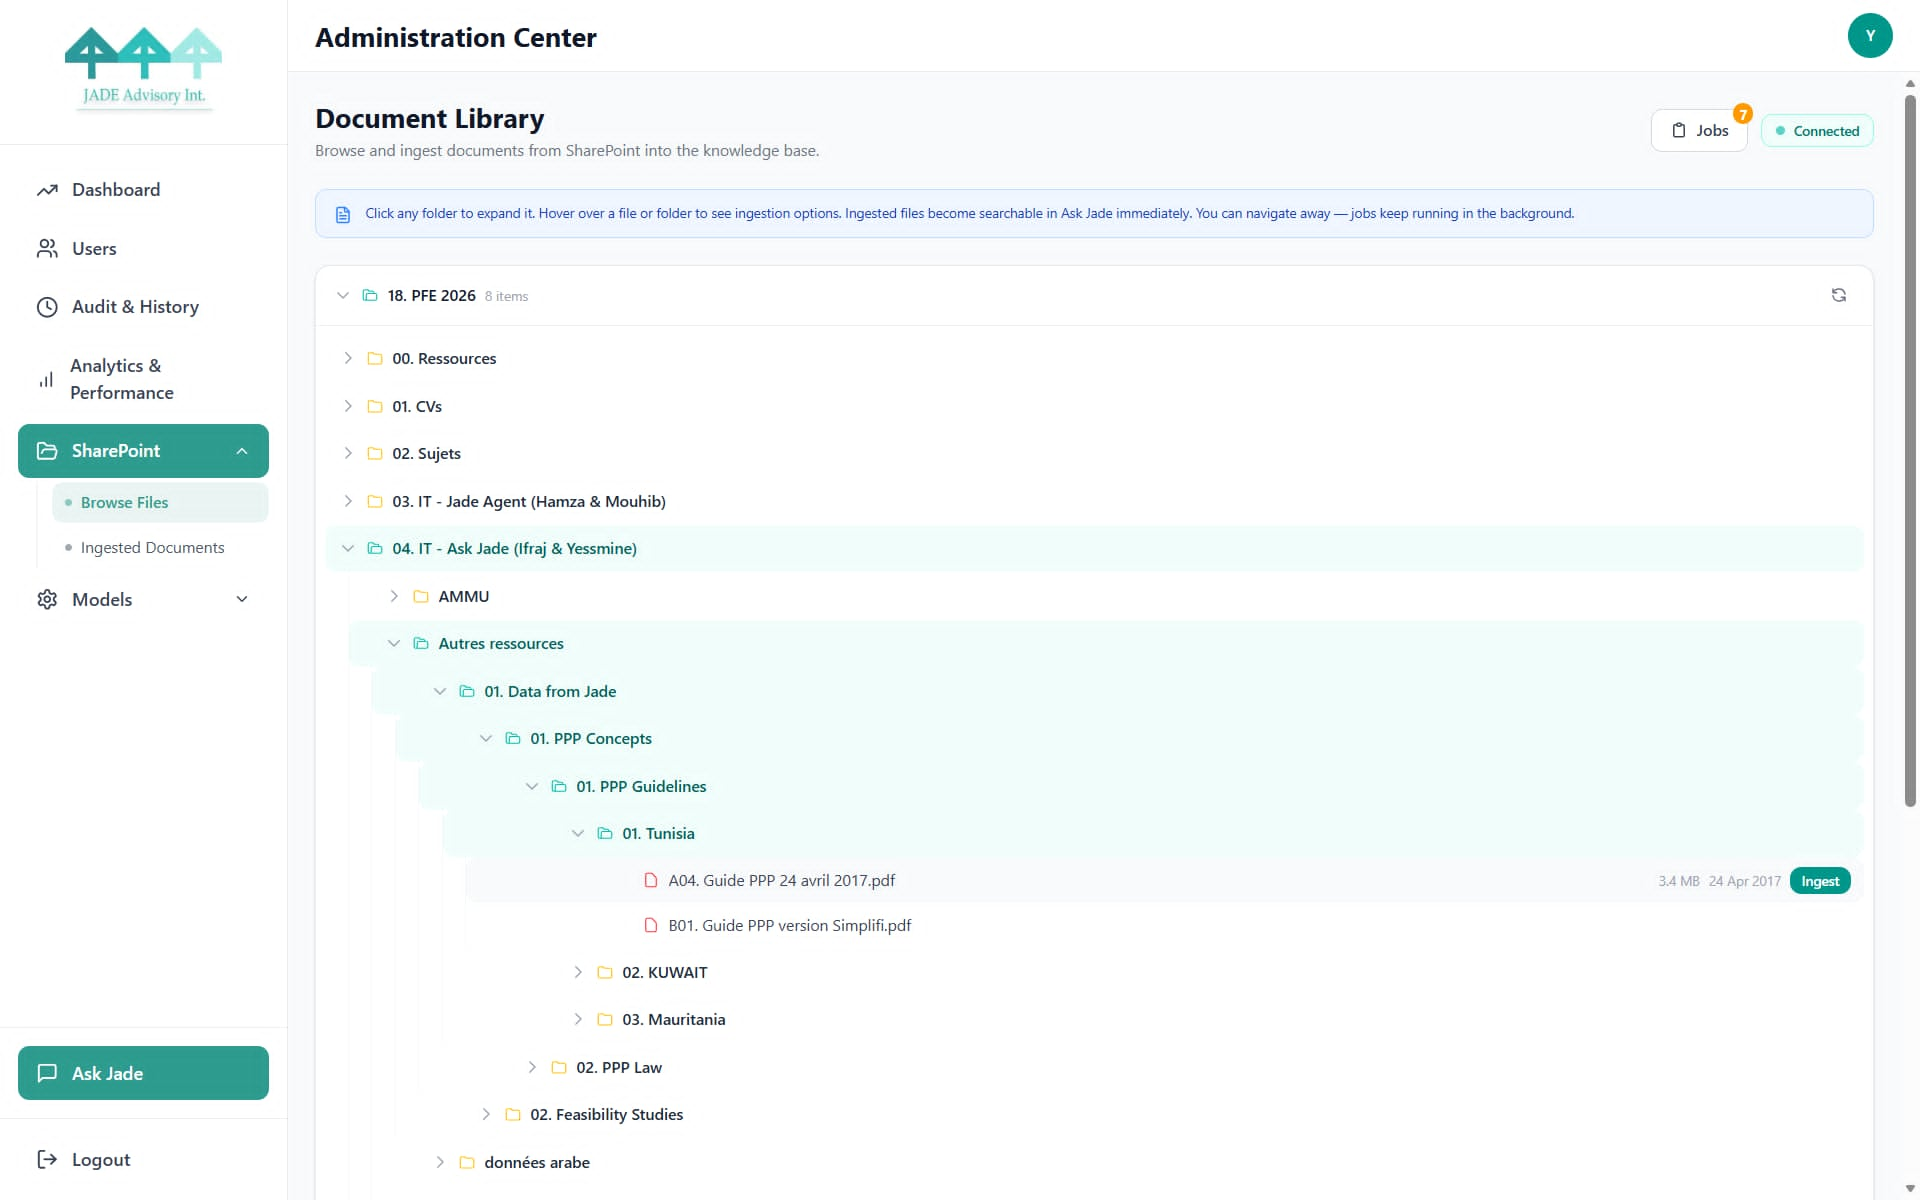
\includegraphics[width=\textwidth]{ingest.jpg}
\caption{Administration Center --- SharePoint file browser}
\label{fig:sharepoint_browser}
\end{figure}

\textbf{Figure~\ref{fig:doc_jobs}} presents the ingestion jobs queue, which tracks
each document through four sequential stages: Queued,
Extracting, Validate, and Indexed. The active
stage is visually highlighted along the progress bar, and a timestamp
records the exact moment processing began. This view gives the Document
Manager full real-time visibility into the pipeline and can be accessed
at any time via the Jobs button without interrupting background
processing.

\begin{figure}[H]
\centering
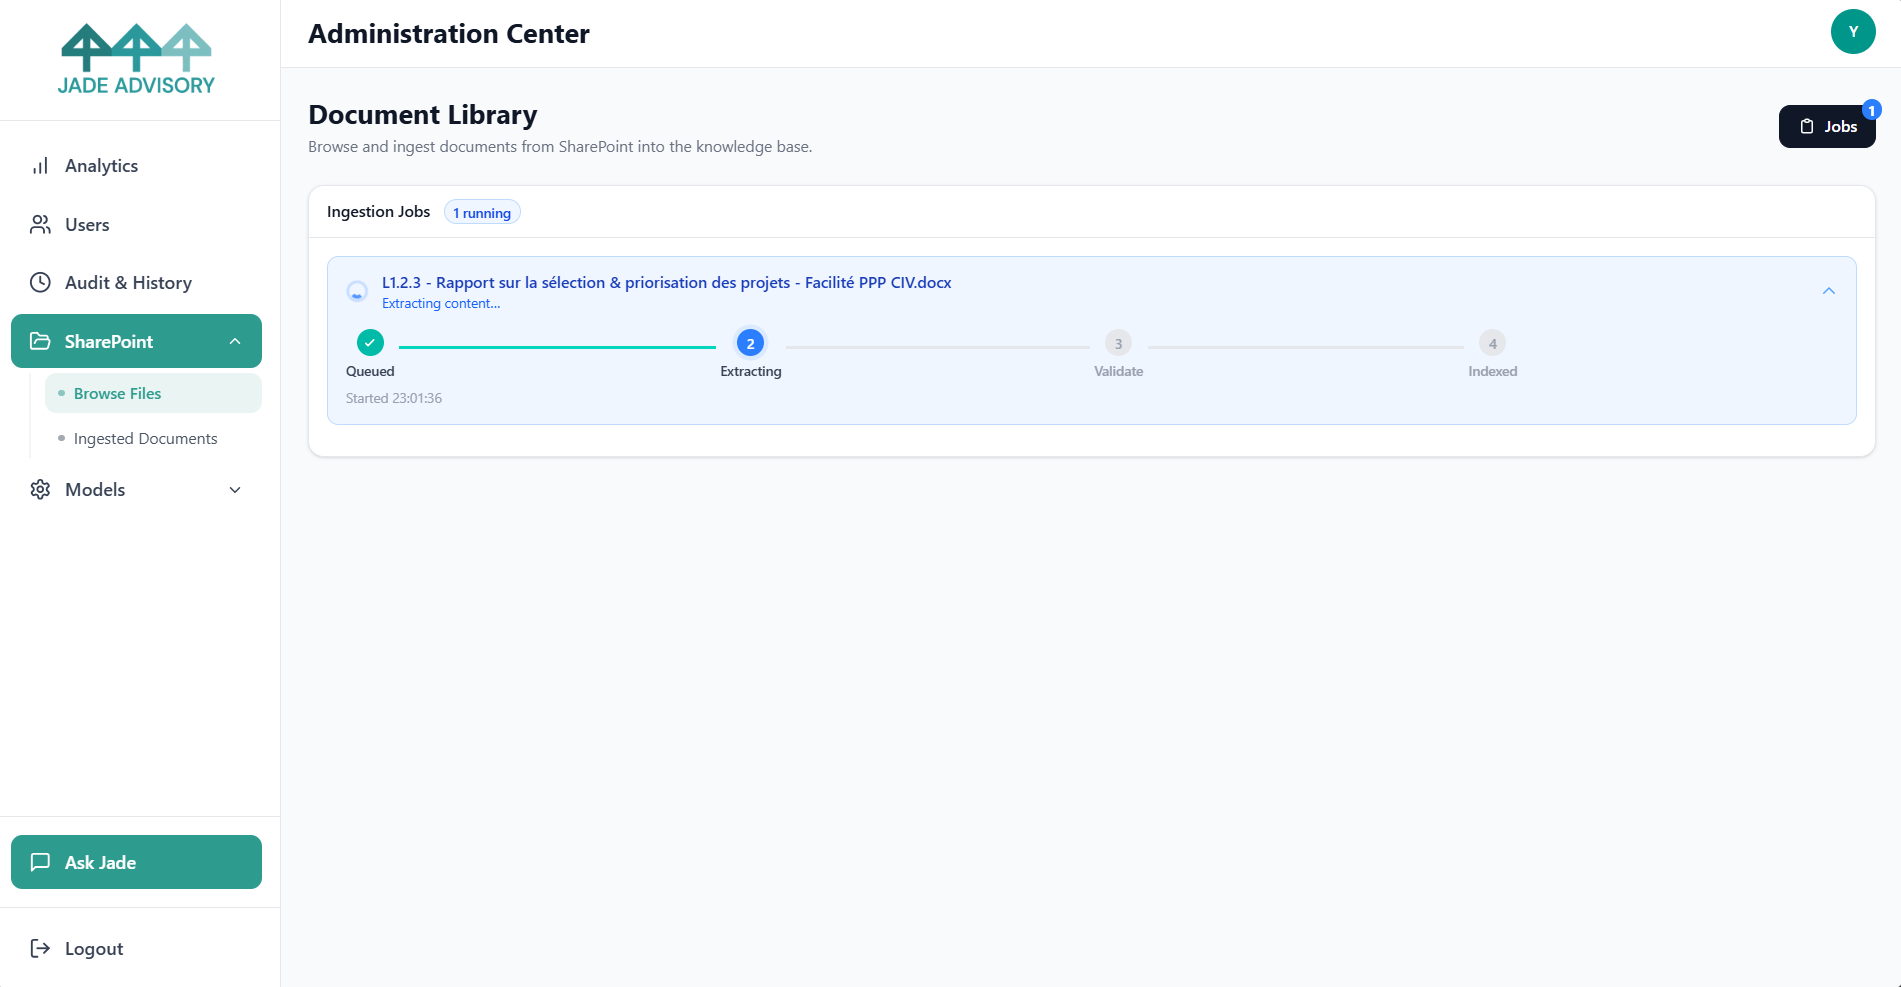
\includegraphics[width=\textwidth]{ingestion_jobs.png}
\caption{Administration Center --- Ingestion jobs queue}
\label{fig:doc_jobs}
\end{figure}

\textbf{Figure~\ref{fig:doc_dashboard}} shows the ingested documents dashboard,
which consolidates all processed documents in a searchable and filterable
table. Three summary counters at the top display the total number of
documents, the number of active documents, and those awaiting validation.
Each row shows the document name, type, associated project, country, the
user who triggered the ingestion, the current status (Active or
Pending Validation), and the ingestion date. From this view, the
Document Manager can edit document metadata, download the original file,
or permanently delete the record using the action icons on the right.

\begin{figure}[H]
\centering
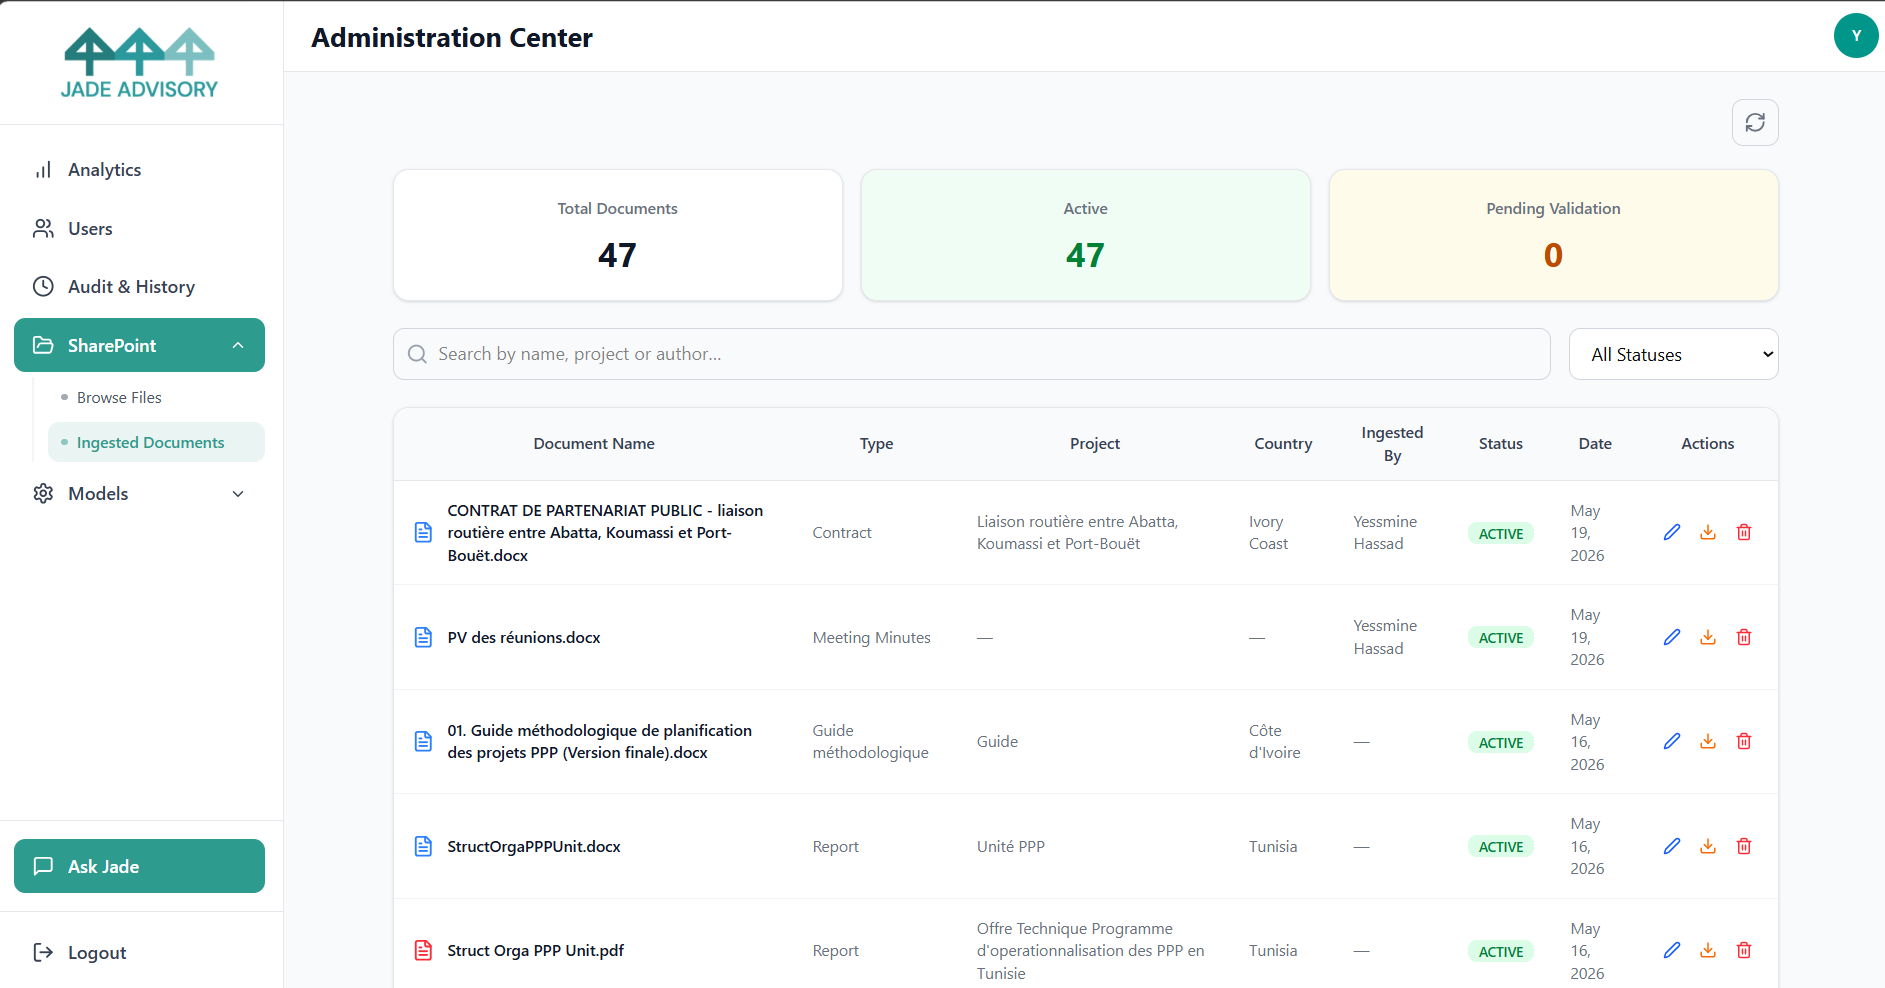
\includegraphics[width=\textwidth]{document_library_ingested.png}
\caption{Administration Center --- Ingested documents dashboard}
\label{fig:doc_dashboard}
\end{figure}

\section{Metadata Interfaces}
\label{annexe:metadata_interfaces}

\textbf{Figure~\ref{fig:edit_metadata}} presents the metadata editing modal,
accessible at any time from the ingested documents dashboard. The form
allows the Document Manager to update any metadata field associated with
an ingested document, including document type, project name, client,
country, year, and sector. Changes are applied immediately upon confirmation.

\begin{figure}[H]
\centering
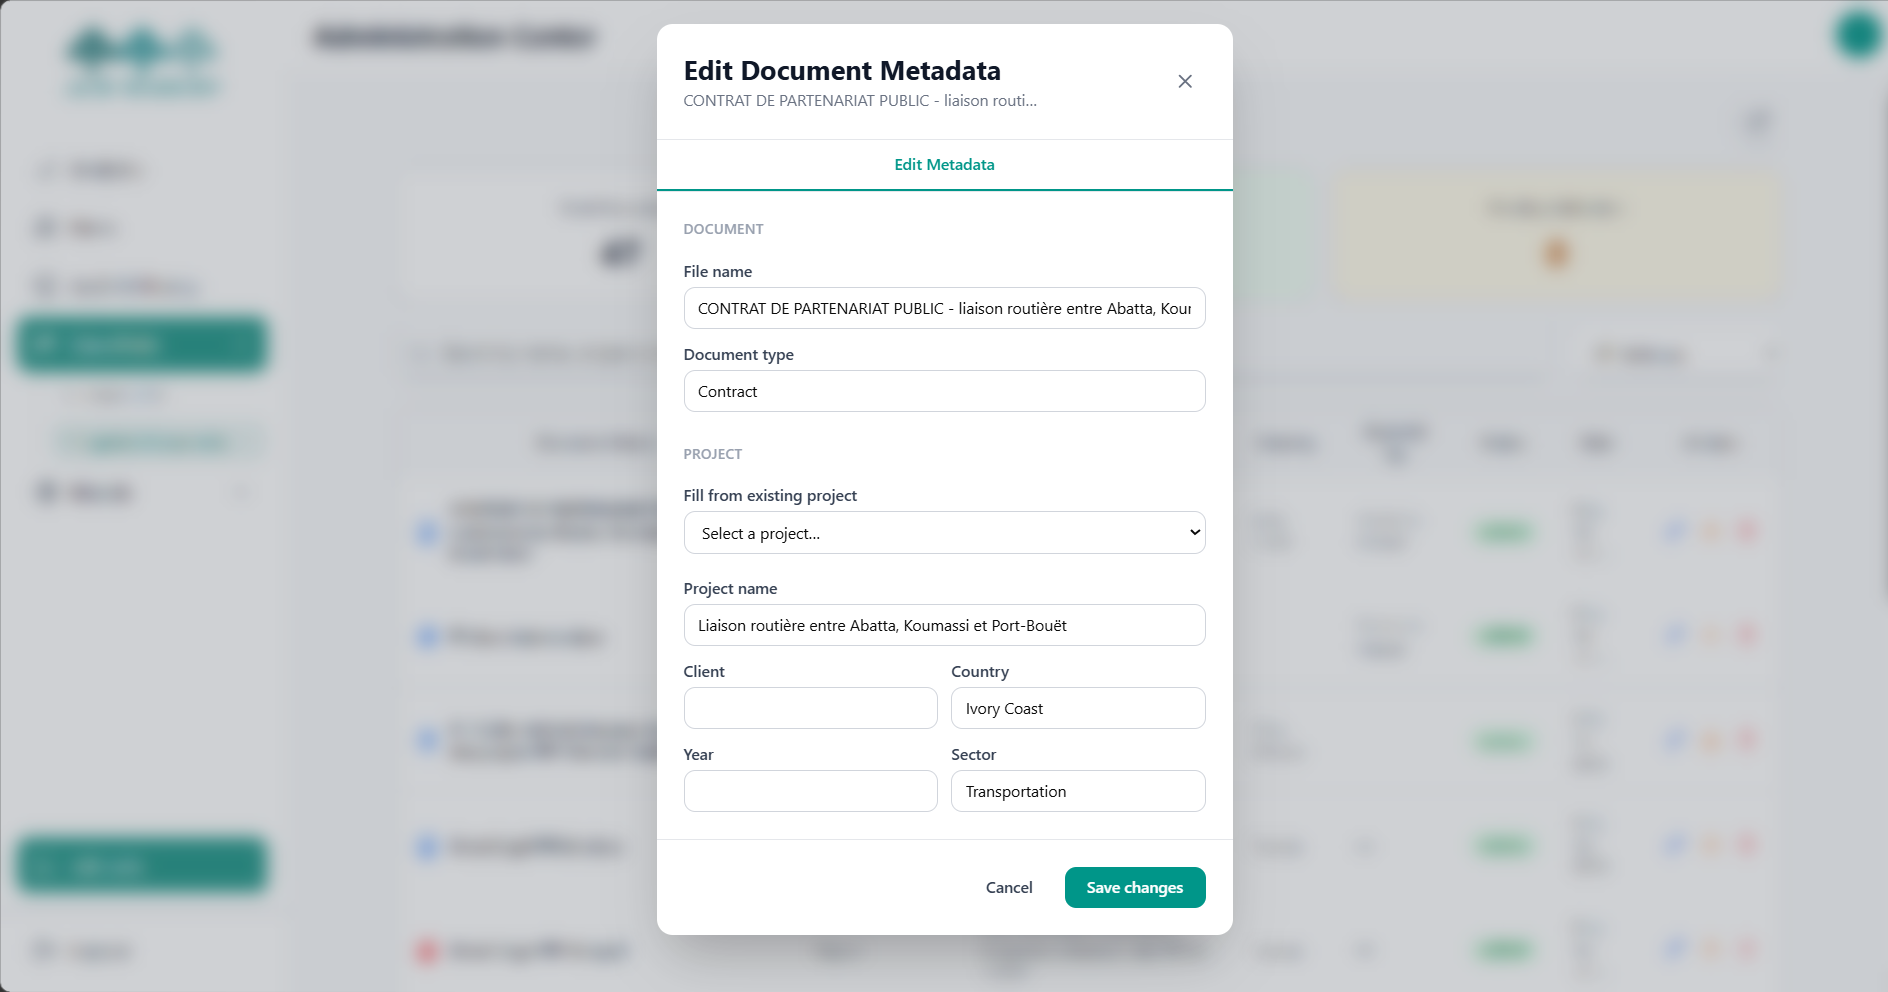
\includegraphics[width=\textwidth]{edit_metadata.png}
\caption{Administration Center --- Metadata editing modal}
\label{fig:edit_metadata}
\end{figure}



\section{User Management Interfaces}
\label{annexe:user_interfaces}

\textbf{Figure~\ref{fig:users_main}} presents the main users dashboard, where
all active accounts are listed in a searchable and filterable table.
Each row displays the user's name, email address, assigned role
(Admin, Document Manager, or Consultant),
current status (Active or Pending), and creation date.
The Administrator can add a new user via the Add User button,
filter accounts by role using the dropdown, or switch to the archived
users view. Per-row action icons allow editing a user's profile,
archiving the account, or deleting it permanently.

\begin{figure}[H]
\centering
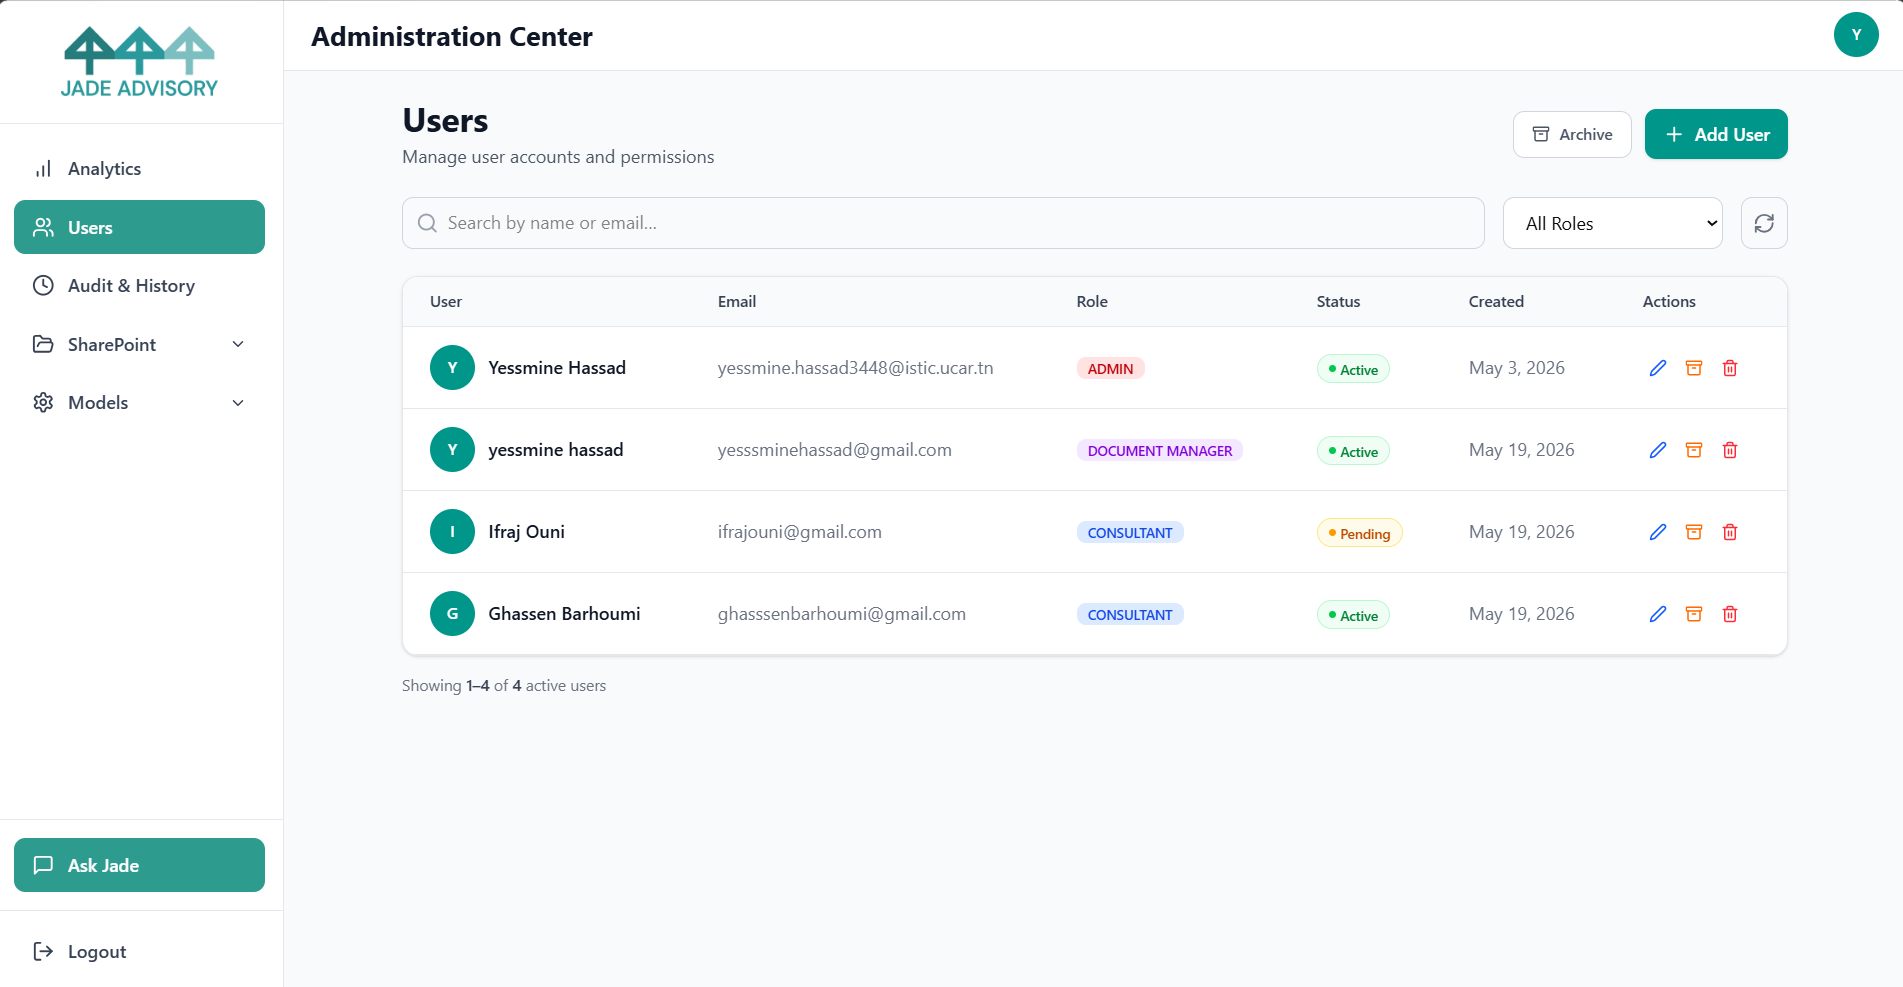
\includegraphics[width=\textwidth]{users_main.png}
\caption{Administration Center --- Users dashboard}
\label{fig:users_main}
\end{figure}

\textbf{Figure~\ref{fig:invite_user}} presents the invite new user modal,
accessible by clicking the Add User button on the dashboard.
The Administrator fills in the new user's first name, last name, email
address, and assigns a role (Admin, Document Manager,
or Consultant). Upon clicking Send Invitation, the
system automatically sends an activation email containing a link for
the user to set their password. The account status remains
Pending until the user completes the activation process.

\begin{figure}[H]
\centering
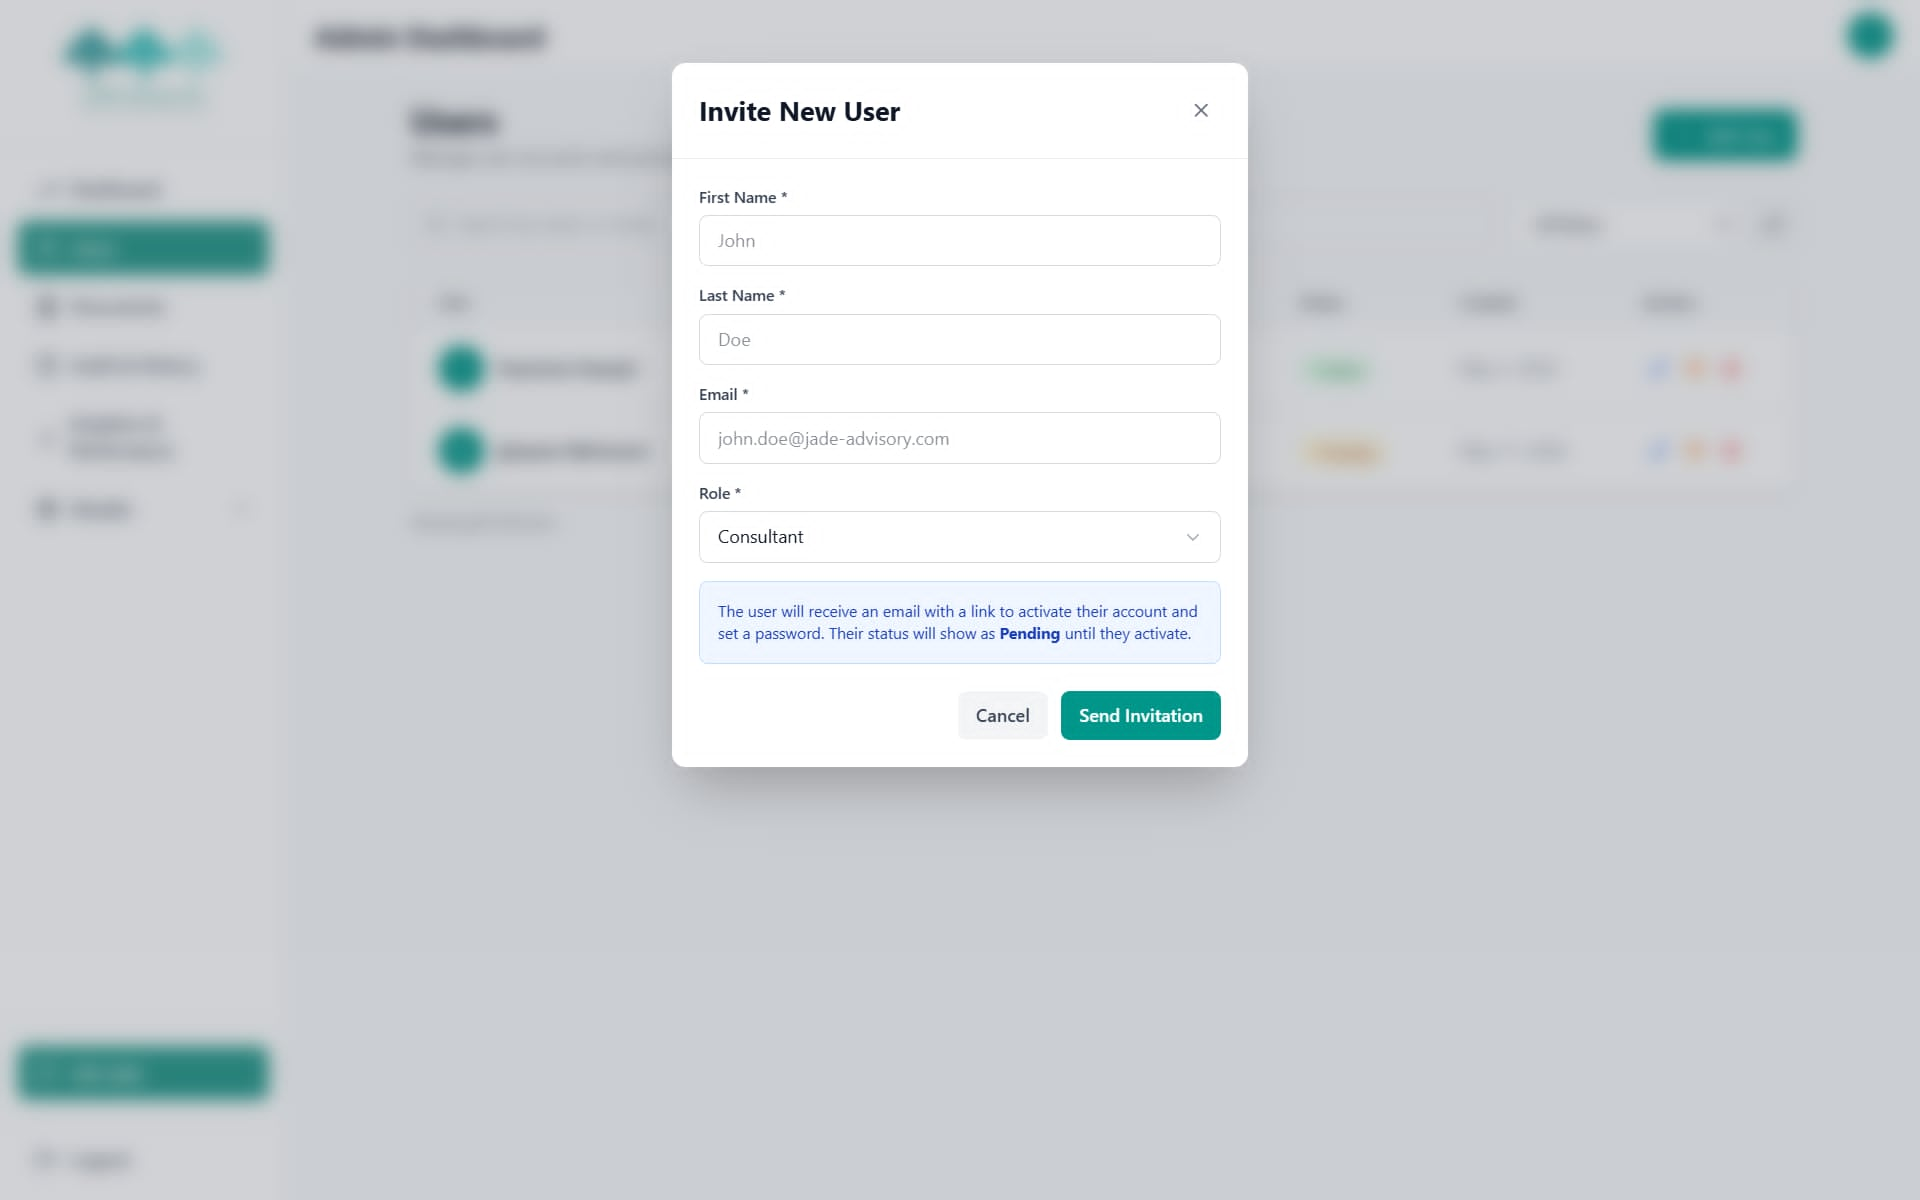
\includegraphics[width=\textwidth]{invite_user.jpg}
\caption{Administration Center --- Invite New User modal}
\label{fig:invite_user}
\end{figure}

\textbf{Figure~\ref{fig:users_archived}} presents the archived users view,
accessible by clicking the Showing Archived toggle on the
dashboard. Archived accounts are displayed in a greyed-out style to
distinguish them from active users, and each entry shows the user's
name, email, role, archived status, and creation date. The Administrator
can restore an account using the restore icon or permanently delete it
using the delete icon.

\begin{figure}[H]
\centering
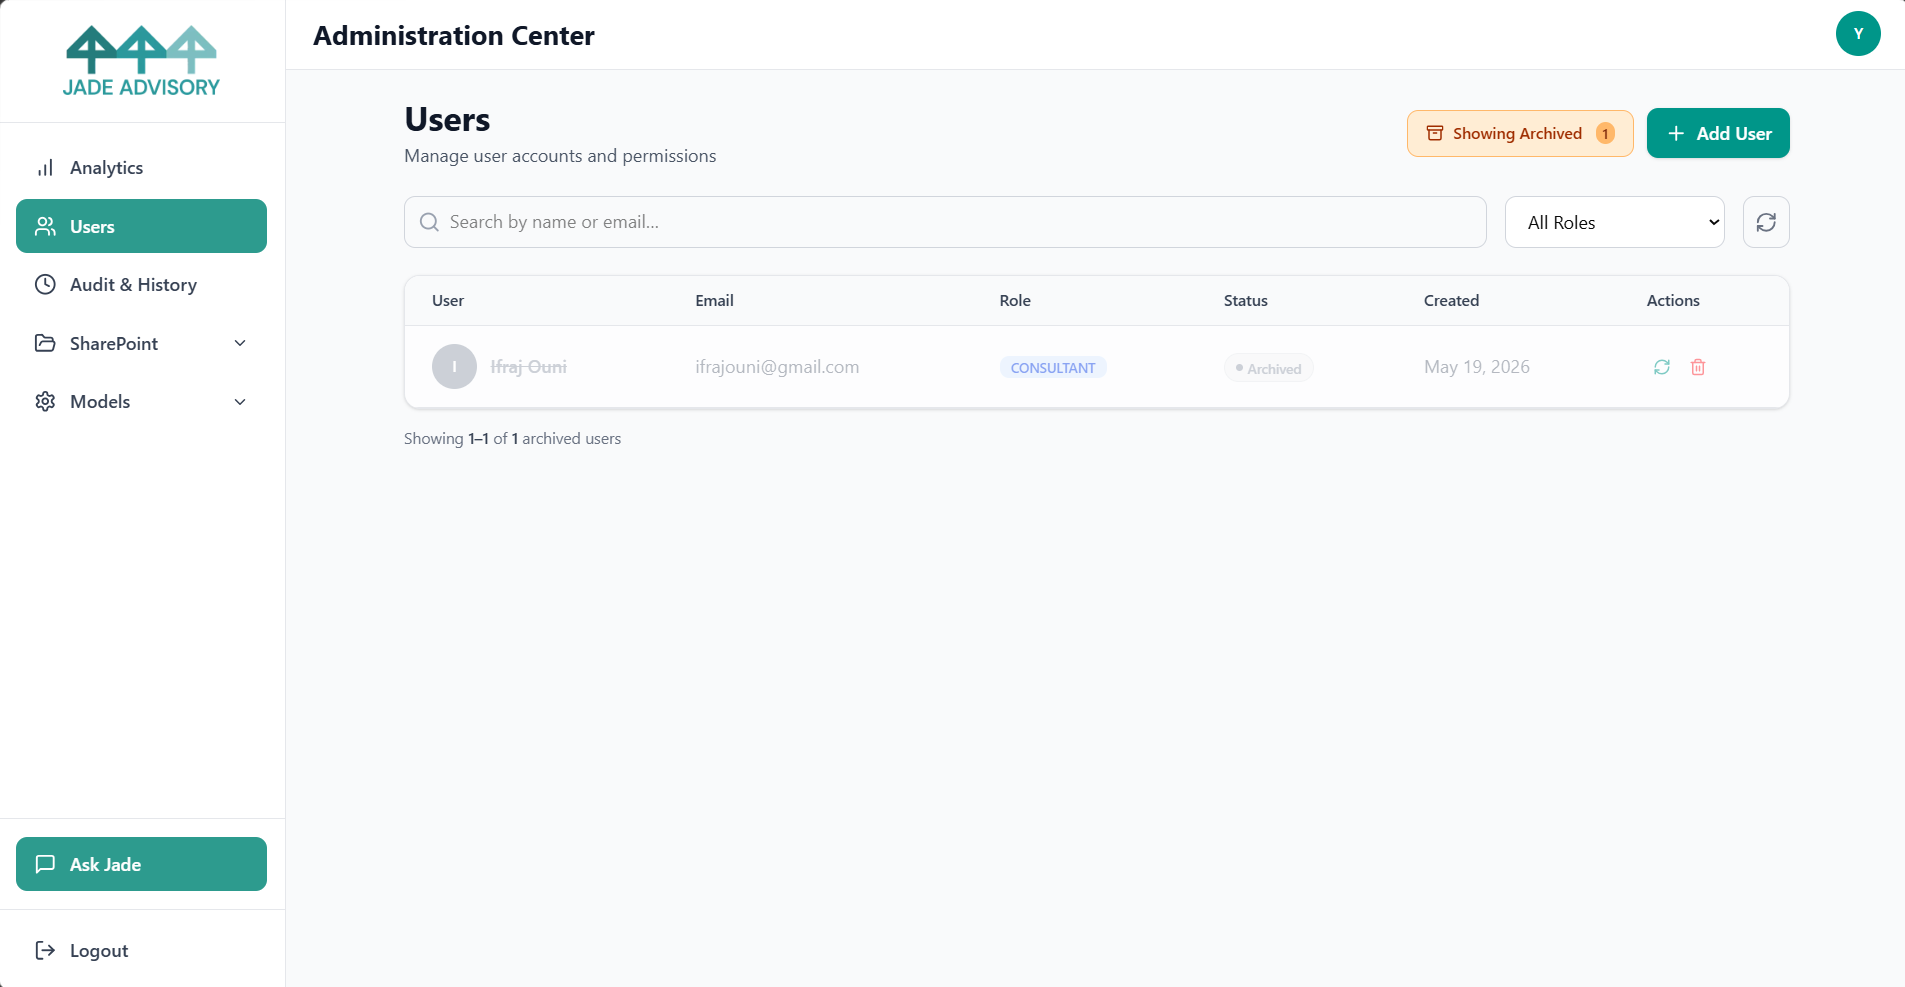
\includegraphics[width=\textwidth]{users_archived.png}
\caption{Administration Center --- Archived users view}
\label{fig:users_archived}
\end{figure}

\textbf{Figure~\ref{fig:edit_profile}} presents the profile editing modal,
accessible by clicking the edit icon on any user row. The form allows
the Administrator to update the user's first name, last name, phone
number, and address. The email field is displayed but locked, as it
cannot be modified after account creation. Changes are applied by
clicking Save Changes.

\textbf{Figure~\ref{fig:edit_password}} presents the password editing modal,
which allows the Administrator to update the password of any user
account. The form requires the current password as confirmation,
followed by the new password (minimum eight characters) and its
confirmation. Clicking Save Changes applies the new password
immediately.

\begin{figure}[H]
\centering
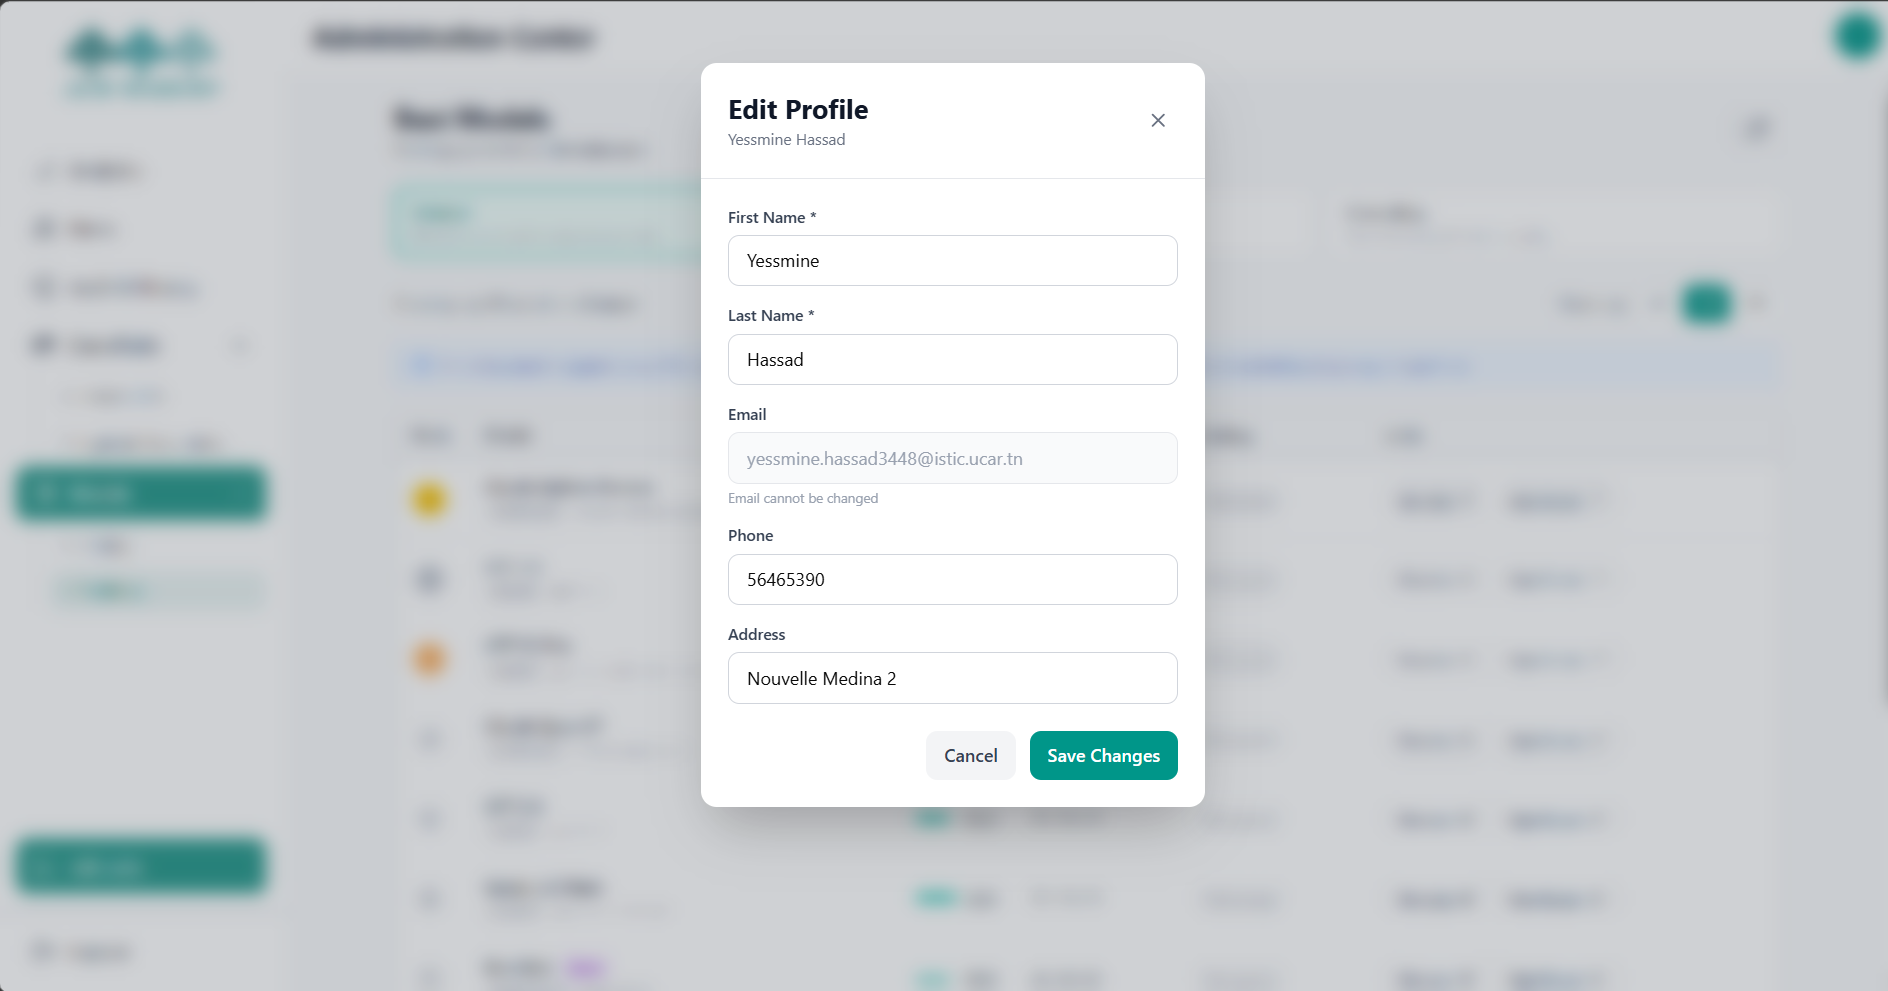
\includegraphics[width=\textwidth]{edit_profile.png}
\caption{Administration Center --- Edit Profile modal}
\label{fig:edit_profile}
\end{figure}



\begin{figure}[H]
\centering
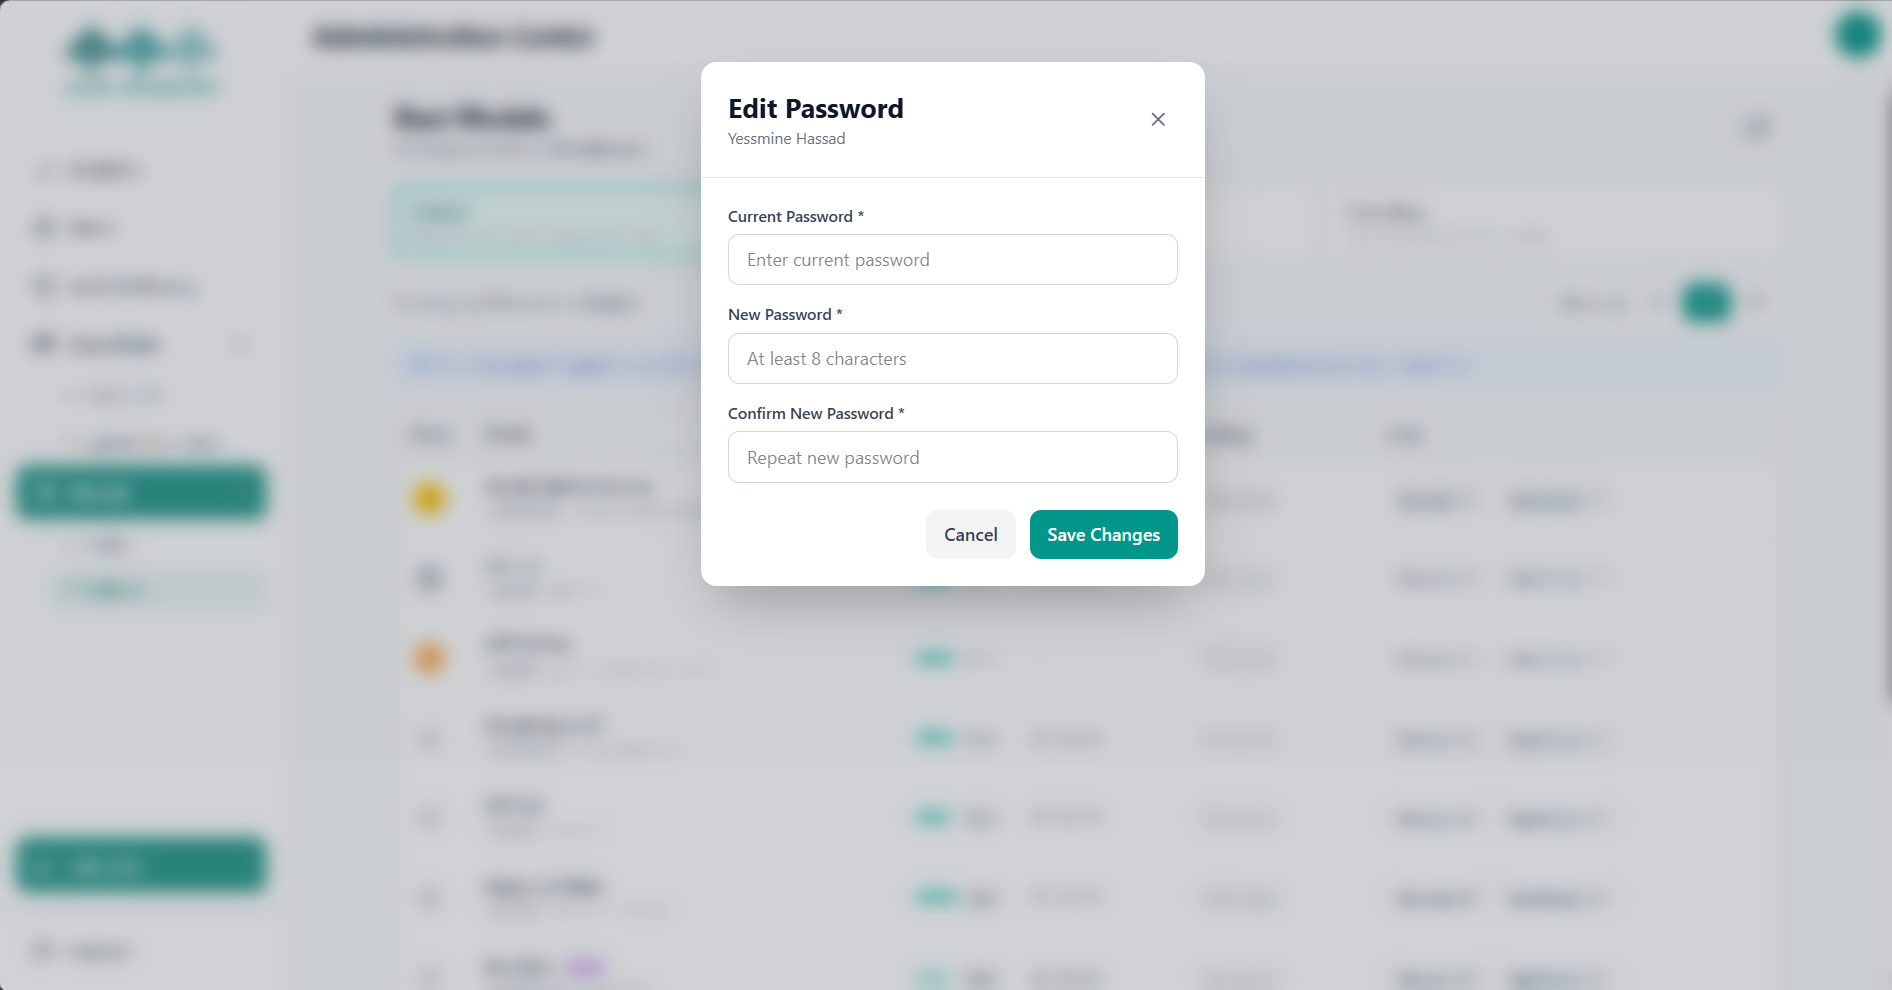
\includegraphics[width=\textwidth]{edit_password.png}
\caption{Administration Center --- Edit Password modal}
\label{fig:edit_password}
\end{figure}



\section{Analytics Dashboard Interfaces}
\label{annexe:analytics_interfaces}

\textbf{Figure~\ref{fig:interface_analytics_costs}} presents the model
performance overview, which displays a bar chart comparing average and
P95 latency across all models, alongside a pie chart showing the
distribution of calls per model. A detailed table below lists, for each
model, the total number of calls, tokens consumed, cumulative cost, and
latency statistics.

\begin{figure}[H]
\centering
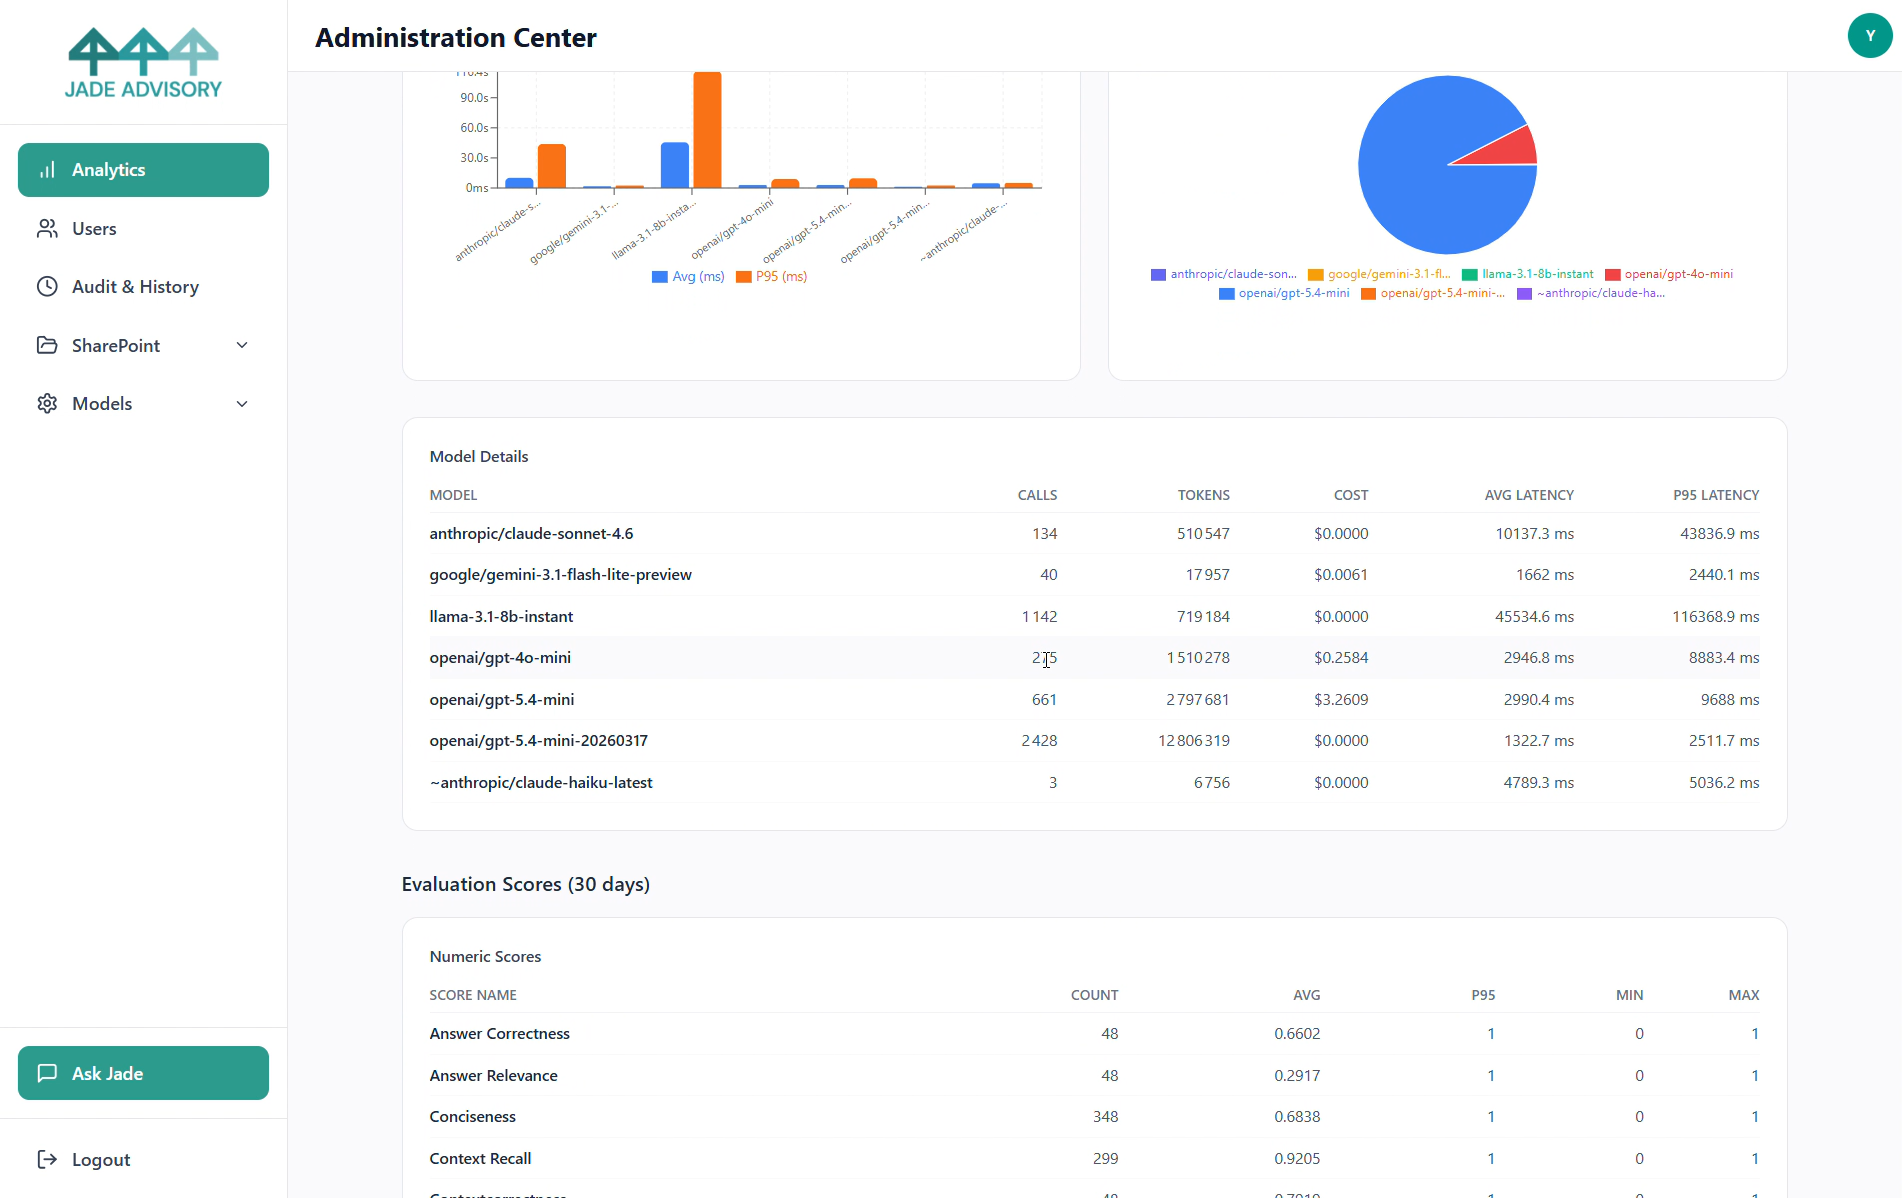
\includegraphics[width=\textwidth]{analytics2.png}
\caption{Administration Center --- Model performance and costs}
\label{fig:interface_analytics_costs}
\end{figure}

\textbf{Figure~\ref{fig:interface_analytics_scores}} presents the evaluation
scores panel, which aggregates LLM-as-a-Judge metrics over the last 30 days.
For each score dimension --- including Answer Correctness, Faithfulness,
Context Recall, Hallucination, and Relevance --- the table reports the
evaluation count, average score, P95 value, and the observed minimum
and maximum, giving administrators a comprehensive view of pipeline
quality over time.

\begin{figure}[H]
\centering
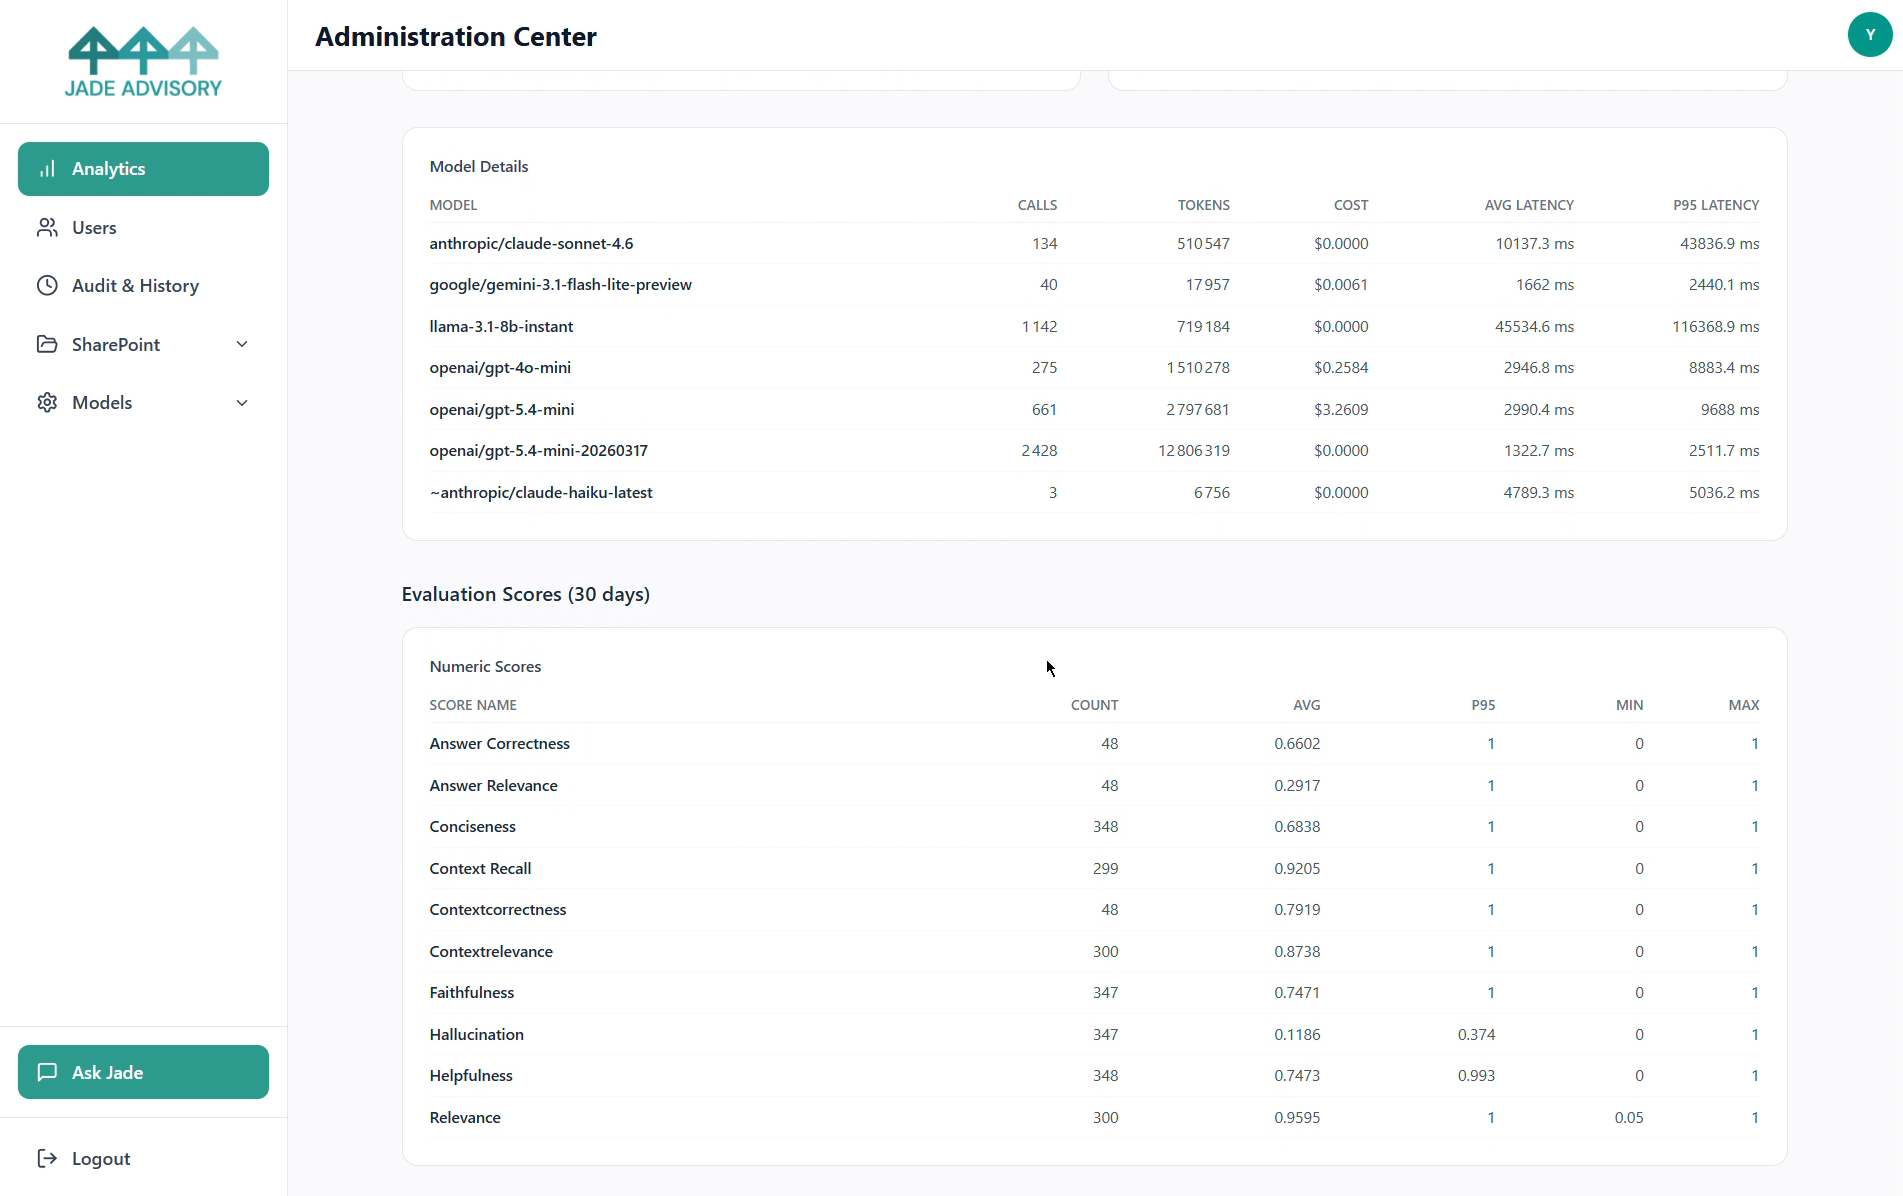
\includegraphics[width=\textwidth]{analytics3.png}
\caption{Administration Center --- Model details and evaluation scores}
\label{fig:interface_analytics_scores}
\end{figure}


\section{Model Management Interfaces}
\label{annexe:models_interfaces}

\textbf{Figure~\ref{fig:your_models}} presents theYour Models view,
accessible by switching to the Your Models tab in the catalog
interface. This view lists only the models currently saved and available
to users in Ask-Jade. Each entry displays the model name and ID, context
window size, input and output prices per million tokens, and the default
status. The model marked as Default is indicated with a
checkmark and is the one automatically assigned when a user opens a new
conversation. Each row also includes a delete icon to remove the model
from the active selection.


\textbf{Figure~\ref{fig:model_rankings}} presents the best models rankings view,
accessible via the Rankings section in the Models menu. Rankings
are powered by llm-stats and are organized into three
domain-specific categories: General (best all-around performance
across tasks), Finance (optimized for financial analysis and
reasoning), and Grounding (factual accuracy and citation quality).
The Administrator can display the top 10, 25, or 50 models per category.
Each row shows the model rank, name and ID, performance score visualized
as a progress bar, minimum price, catalog availability status, and direct
links to the model's page on llm-stats.com and OpenRouter for
further reference before adding it to the active selection.

\begin{figure}[H]
\centering
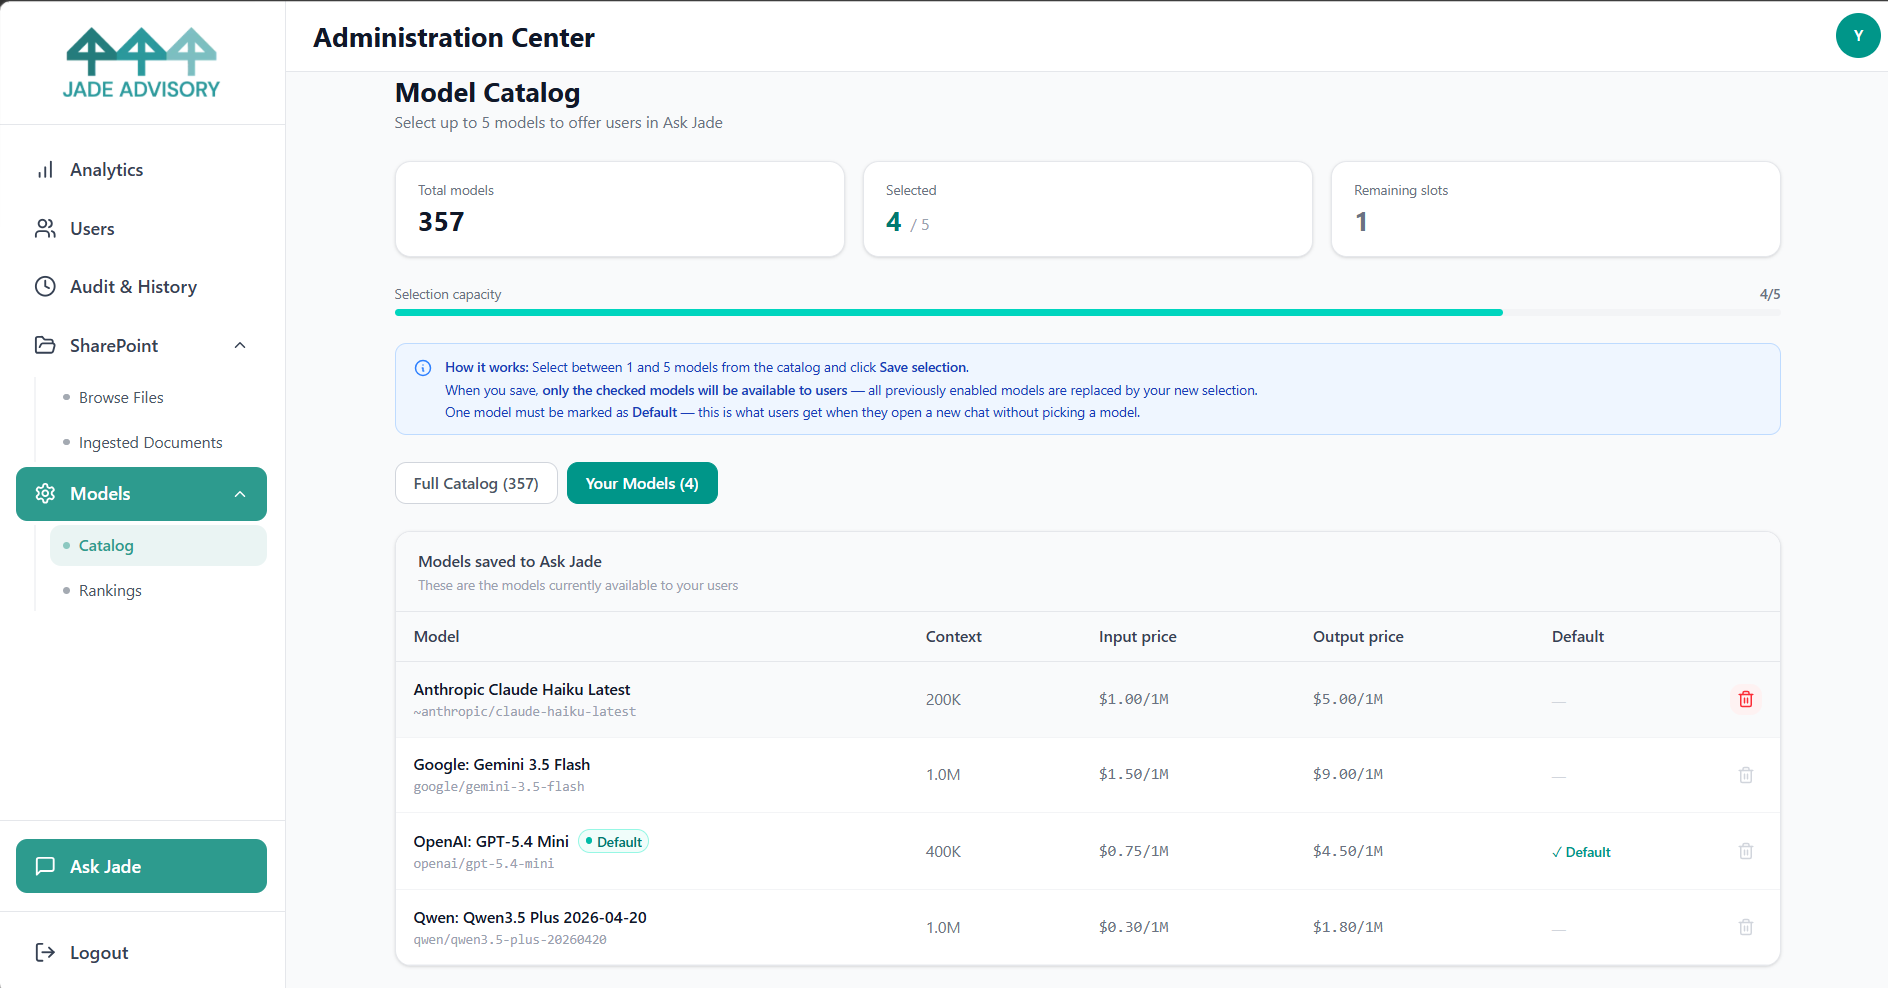
\includegraphics[width=\textwidth]{your_models.png}
\caption{Administration Center --- Active models saved to Ask-Jade}
\label{fig:your_models}
\end{figure}



\begin{figure}[H]
\centering
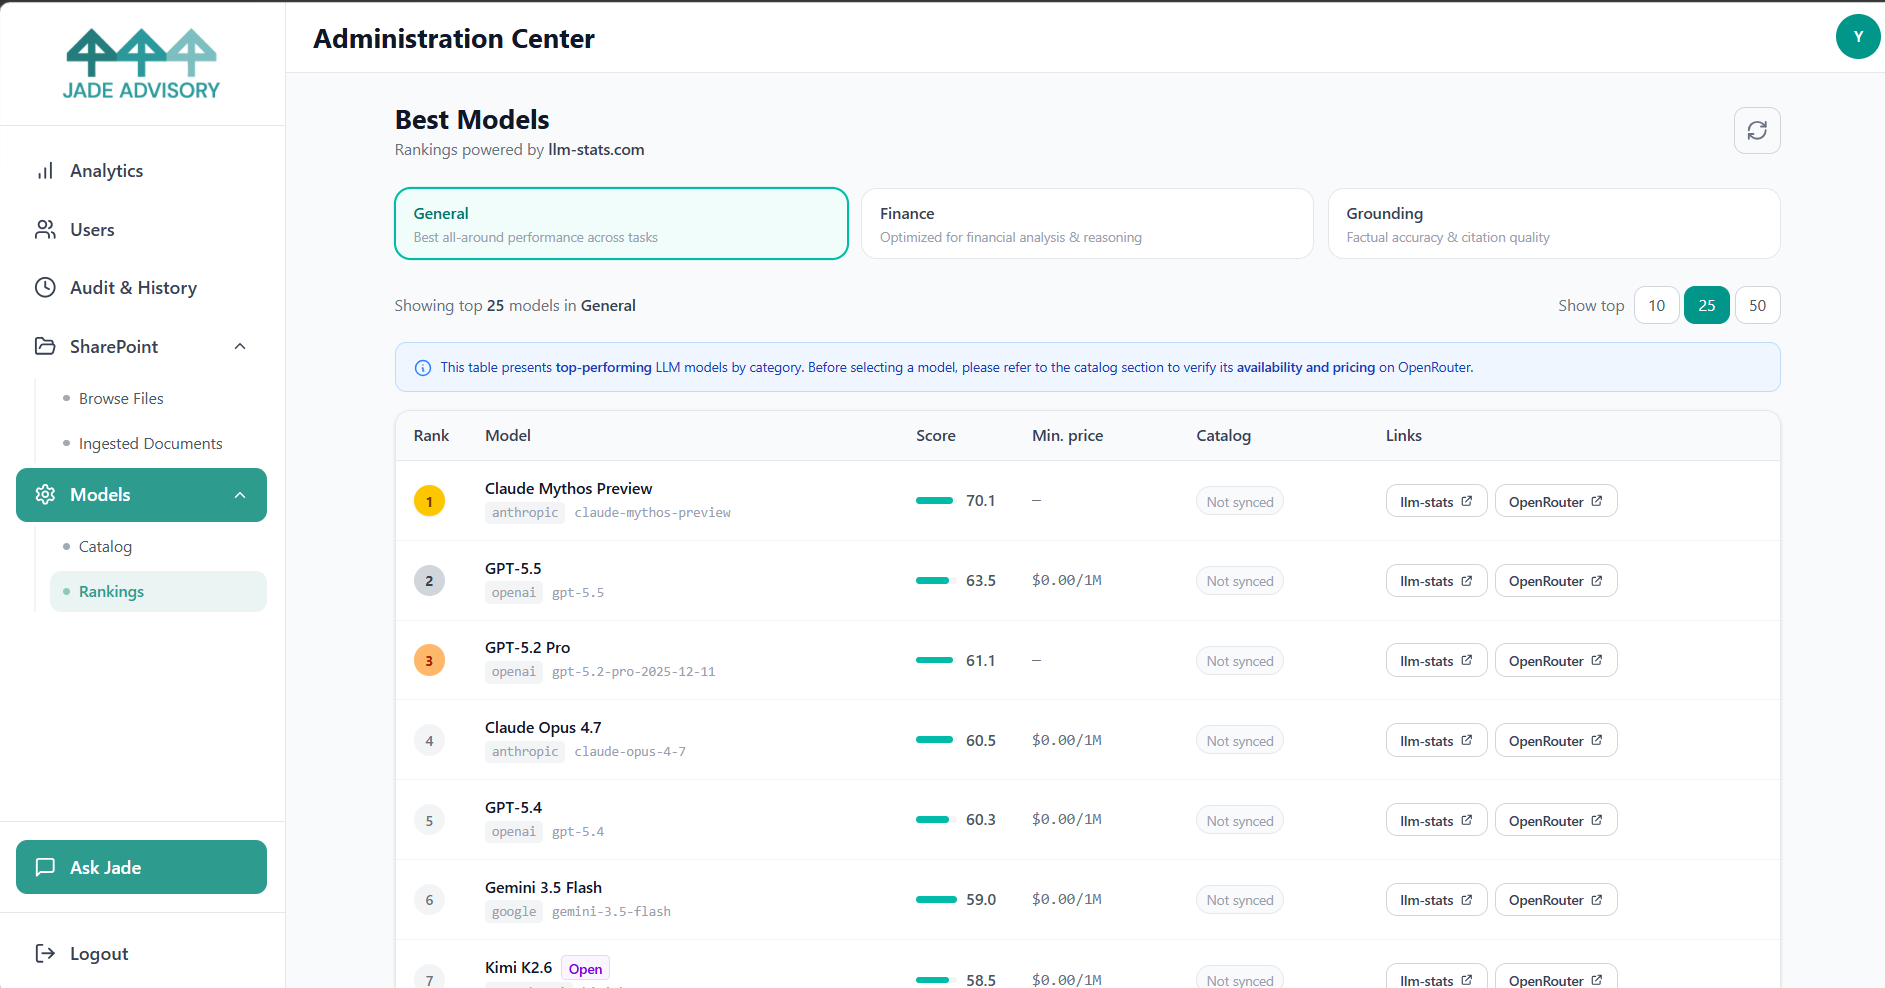
\includegraphics[width=\textwidth]{model_rankings.png}
\caption{Administration Center --- Best models rankings}
\label{fig:model_rankings}
\end{figure}



% ─── Annexe C : Diagrammes de séquence ───────────────────────────────────
\chapter{Sequence Diagrams}
\label{annexe:seq_users}

\section{Manage Users Sequence Diagram}
\label{annexe:seq_manage_users}

\textbf{Figure~\ref{fig:seq_manage_users}} presents the complete sequence diagram
of the Manage Users use case, illustrating the interactions between the
Administrator, the system interface, and the backend across all user
management operations, including adding, editing, archiving, restoring,
and deleting user accounts.

\begin{figure}[H]
\centering
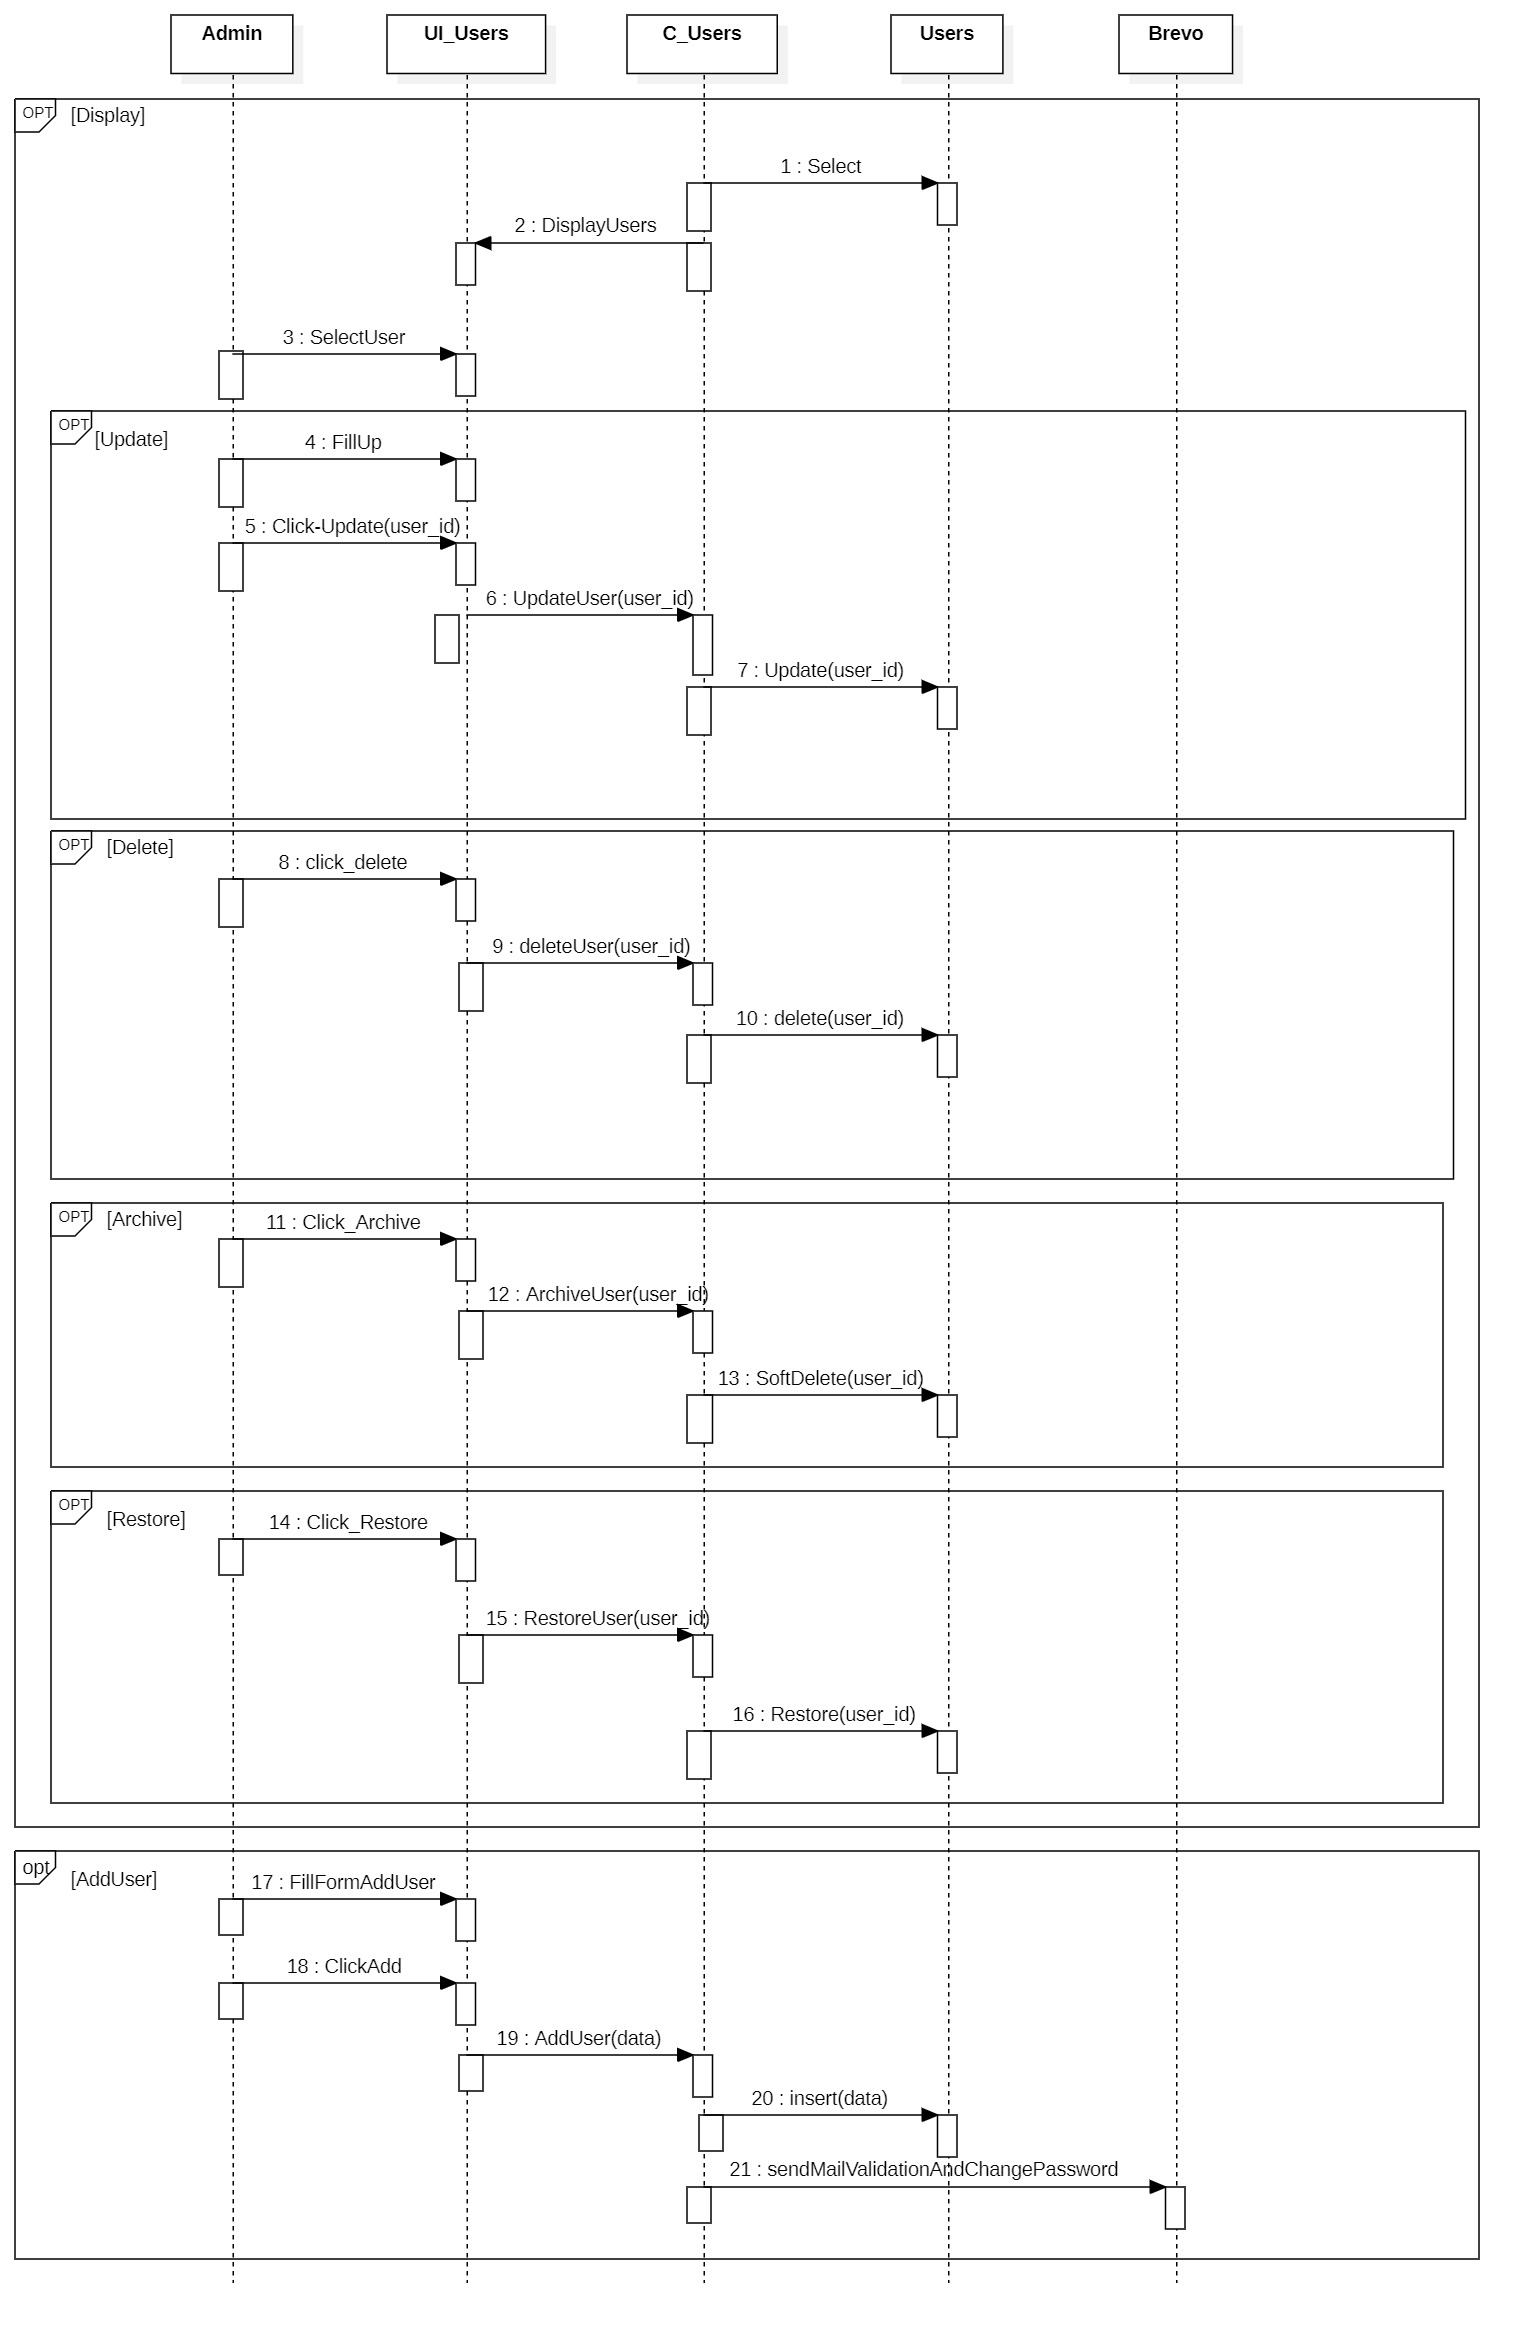
\includegraphics[width=\textwidth]{SequenceDiagramUsers1.jpg}
\caption{Sequence Diagram --- Manage Users Use Case}
\label{fig:seq_manage_users}
\end{figure}











% ─── Annexe D : Generation Prompt ────────────────────────────────────────
\chapter{Answer Generation Prompt}
\label{annexe:generation_prompt}

This appendix presents the full prompt submitted to the LLM at the answer generation stage.

\nopagebreak
\begin{center}
\begin{minipage}{0.92\textwidth}
\begin{Verbatim}[frame=single, rulecolor=\color{gray!60}, fontsize=\footnotesize]
You are a PPP (Public-Private Partnership) expert assistant
for Jade Advisory. The context provided is from Jade
Advisory's Document Library.
## CORE INSTRUCTION
- Answer the QUESTION directly, precisely, and strictly
  based on the provided Context.
- Focus ONLY on what is asked. Ignore irrelevant text.
- Include examples from the context when relevant.
- Do not write an introduction.
- If the context presents a table, return the table with
  the columns and rows related to the answer.
- If asked about a value in a Financial Model, give the
  exact value -- do NOT invent.
## LANGUAGE RULE
- Detect the language of the QUESTION and respond in that
  SAME language, regardless of the context language.
## CONCISENESS & STYLE RULES
- Be extremely concise. Remove all redundancies.
- Do NOT include introductory phrases such as
  "Based on the context...".
- Start directly with the first factual element.
- Use structured tables or bullet points when appropriate.
## FORMATTING RESTRICTIONS
- Generate only: Text, Markdown Tables, or Mermaid diagrams.
- For any other format request, reply:
  "I can only generate text, tables, and Mermaid diagrams."
## FALLBACK
- If the context does not contain the information needed,
  reply exactly:
  "I could not find relevant information about this in
  the available documents."
---------------------
Question: {query_str}
---------------------
Context:  {context_str}
---------------------
Answer (in the same language as the Question):
\end{Verbatim}
\end{minipage}
\end{center}